\chapter{View Points}
\label{sec:view_points} 

The 'View Points' tab displays existing view points, allows selection, stepping and editing of view points. Additionally, view points can be imported, removed and exported.

\begin{figure}[H]
    \hspace*{-2.5cm}
    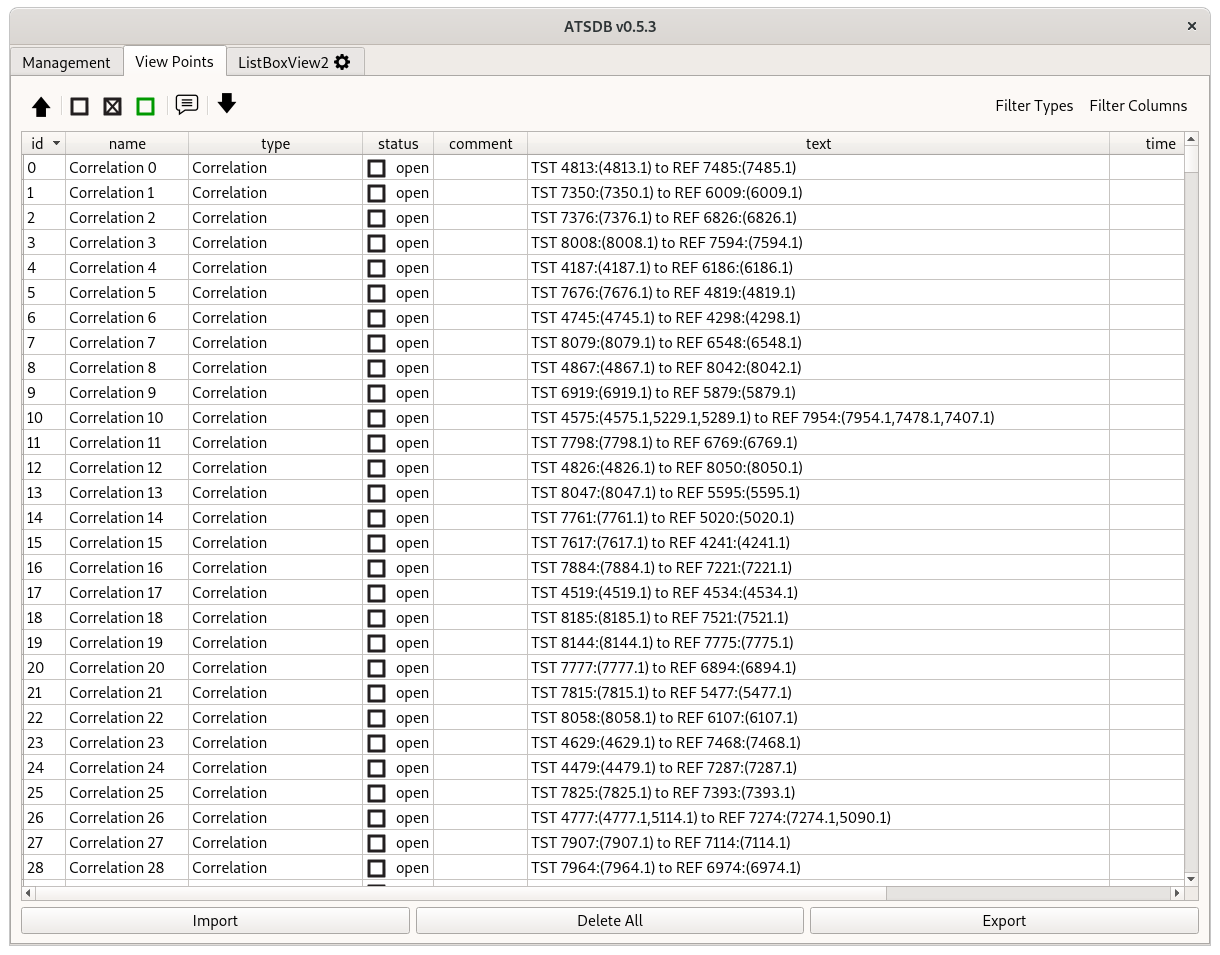
\includegraphics[width=19cm]{../screenshots/view_points.png}
  \caption{View Points Tab}
\end{figure}

At the top, a toolbar is shown. In the middle, a table showing all existing view points exists. At the bottom, general function buttons exist. \\

\section{View Point}

A view point is a point of interest in the data persisted in the database. It has the following attributes:

\begin{center}
 \begin{table}[H]
  \begin{tabularx}{\textwidth}{ | l | X | }
    \hline
    \textbf{Key} & \textbf{Value Description} \\ \hline
    id & Identifier, as number \\ \hline
    type & Type, e.g. 'Short track', 'Extra track', 'Content deviation X'  \\ \hline
    status & Editable status, e.g. 'open', 'closed', 'todo' \\ \hline
    comment & Editable user comment \\ \hline
    text & Description text \\ \hline
    position\_latitude & Center position WGS-84 latitude \\ \hline
    position\_longitude & Center position WGS-84 longitude \\ \hline
    position\_window\_latitude & Geographic window size in WGS-84 latitude  \\ \hline
    position\_window\_longitude & Geographic window size in WGS-84 longitude  \\ \hline
    time & Center time  \\ \hline
    time\_window & Time window size \\ \hline
    db\_objects & List of DBObjects to load \\ \hline
    filters & List of filters defining which data to load \\ \hline
    dbo\_context\_variables & List of extra content DBOVariables to load and display \\ \hline
\end{tabularx}
\end{table}
\end{center}
\ \\

Not all attributes are shown in the table, since some are more processing related than information relative to the user. \\

Also, additional attributes can be shown. If other additional attributes exist in the view point information, they are automatically shown in the table. For additional information please refer to \nameref{sec:view_points_custom_attributes}. \\

When a view point is selected, the dataset defined by the view point is loaded automatically and the active Views show the relevant data. Using the elements described in the following sections a user can quickly step through view points, assess the information shown and change status and comment information. \\

Please \textbf{note} that changes to view points are only saved to the database on correct application shutdown.

\section{Toolbar}

\begin{table}[H]
  \center
  \begin{tabular}{ | l | l | l |}
    \hline
    \textbf{Icon} & \textbf{Text} &  \textbf{Description} \\ \hline
    
\includegraphics[width=0.5cm,frame]{../../data/icons/up.png} & Select Previous [Up] & Steps to the previous view point \\ \hline
    
\includegraphics[width=0.5cm,frame]{../../data/icons/not_recommended.png} & Set Selected Status Open [O] & Sets the current view point to status 'open' \\ \hline
    
\includegraphics[width=0.5cm,frame]{../../data/icons/not_todo.png} & Set Selected Status Closed [C] & Sets the current view point to status 'closed' \\ \hline
    
\includegraphics[width=0.5cm,frame]{../../data/icons/todo.png} & Set Selected Status ToDo [T] & Sets the current view point to status 'todo' \\ \hline
    
\includegraphics[width=0.5cm,frame]{../../data/icons/comment.png} & Edit Comment [E] & Edits the current view points status \\ \hline
    
\includegraphics[width=0.5cm,frame]{../../data/icons/down.png} & Select Next [Down] & Steps to the next view point \\ \hline
    & Filter Types & Opens menu for filtering based on type \\ \hline
    & Filter Columns & Open menu for hiding/showing columns \\ \hline    
  \end{tabular}
  \caption{Toolbar Actions}
\end{table}
\ \\

All of the actions can be triggered using the listed keyboard shortcut in the square brackets. Up/Down refers to the keyboard arrows.

\section{Table}

\begin{figure}[H]
    \hspace*{-2cm}
    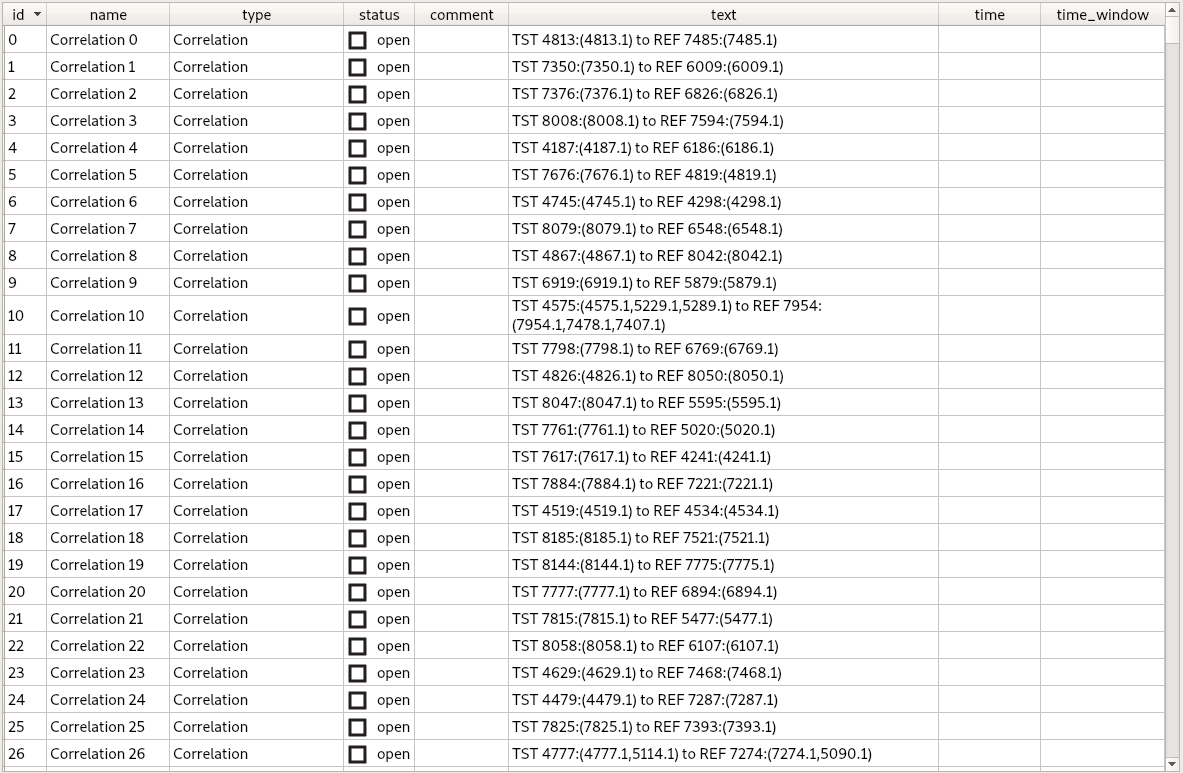
\includegraphics[width=18cm,frame]{../screenshots/view_points_table.png}
  \caption{View Points Table}
\end{figure}

In the view points table, all view points are listed, each one in a seperate row. Columns can be used for ordering (simply click on the column name), and resized as wanted. \\

A click on a view point selects it, which highlights the row.

\begin{figure}[H]
    \hspace*{-2cm}
    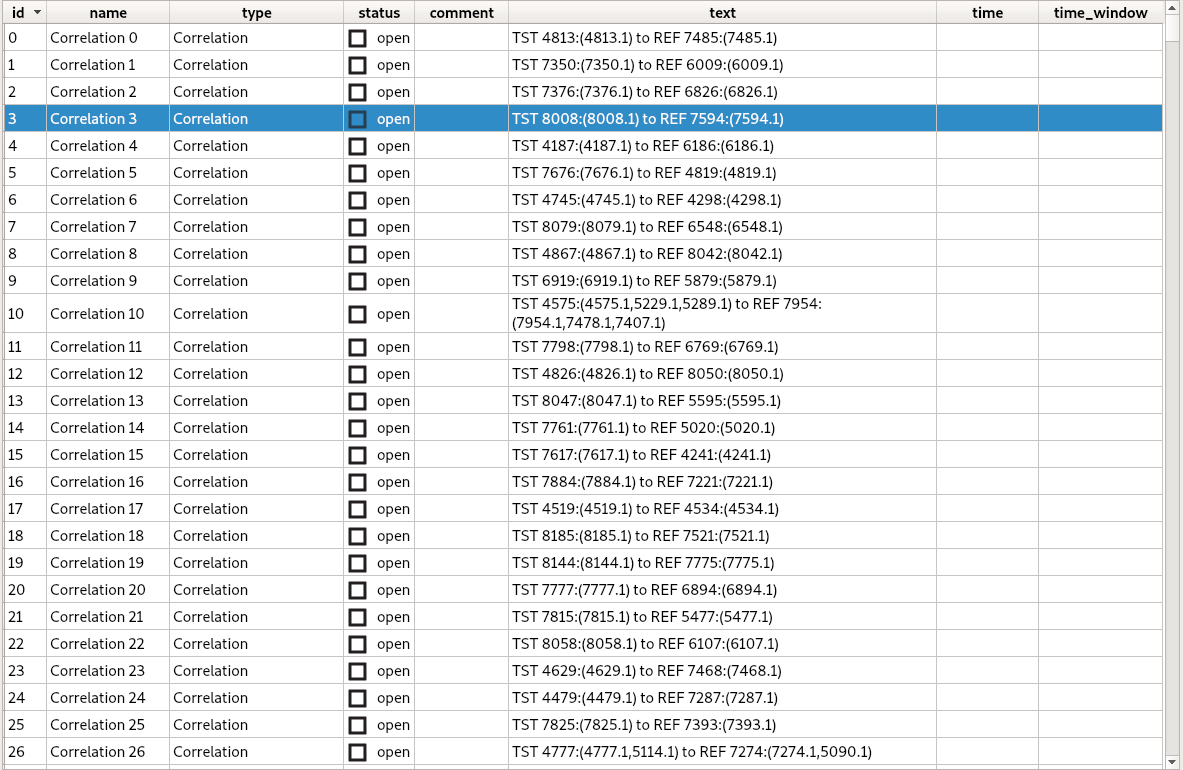
\includegraphics[width=18cm,frame]{../screenshots/view_points_table_selected.png}
  \caption{View Points Table: Selected View Point}
\end{figure}

This automatically triggers loading of the data and display in the existing Views. \\

The status can only be set using the toolbar buttons or keyboard shortcuts, while editing the comment can also be triggered by a double-click on the respective cell.

\section{Function Buttons}

There exist 3 buttons for general functions:

\begin{itemize}  
\item Import: Imports a view point file selected by the user (only recommended if no view points are already defined)
\item Delete All: Deletes all existing view points
\item Export: Exports all existing view points as a view point file
\end{itemize}
\ \\

\section{Stepping View Points}

\subsection{Management Tab} 
When selecting a new view point, the information set in the 'db\_objects' attribute is used to select which DBObjects are loaded. The 'filters' attribute to set the filter active flags and respective conditions. After that, a loading process is triggered. \\

\subsection{Data Selection}

When the loading process is finished, data is automatically selected using the 'time' and 'time\_window' attributes.

\subsection{ListBox View} 

\begin{figure}[H]
    \hspace*{-2cm}
    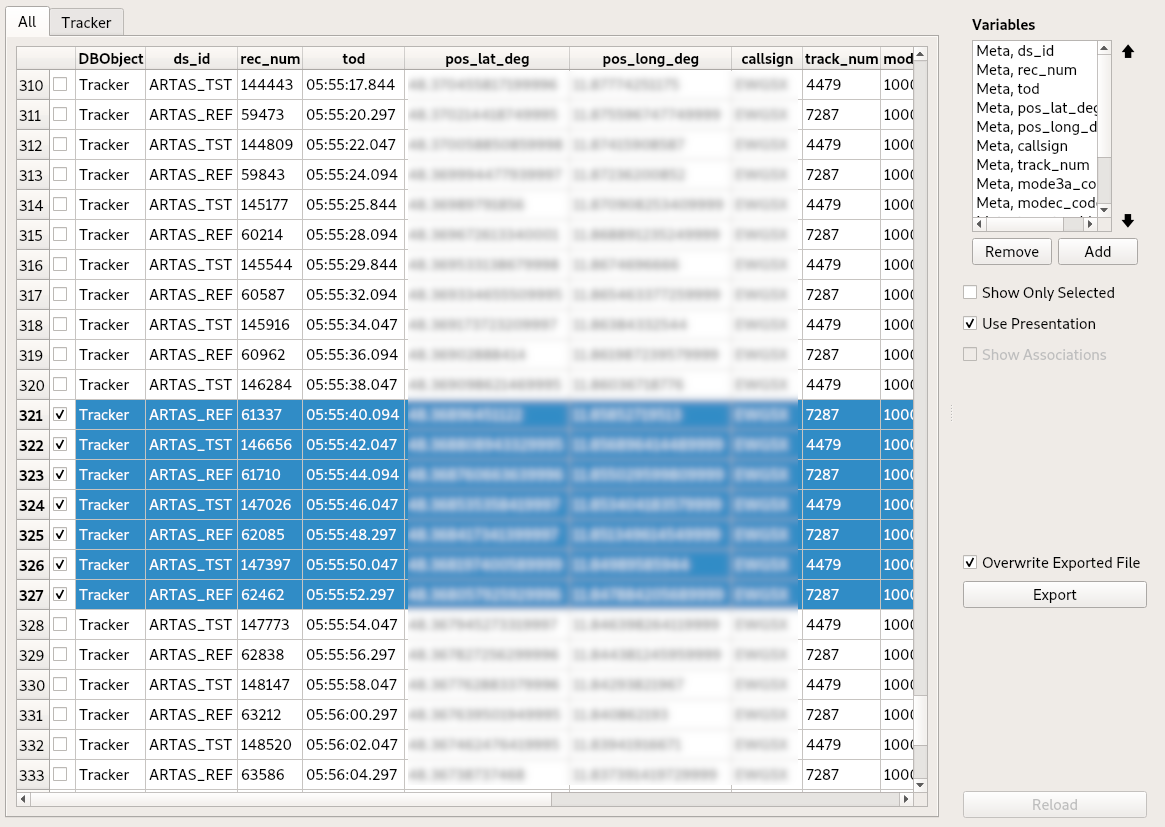
\includegraphics[width=18cm,frame]{../screenshots/view_points_listbox_selected.png}
  \caption{View Points ListBox View: Selected View Point}
\end{figure}

In the ListBox View, the variables set in the 'dbo\_context\_variables' attribute are added temporarily to the list of variables. Loaded data is presented as always. When the loading process is finished, selected data is highlighed.


\subsection{OSGView}

\begin{figure}[H]
    \hspace*{-2cm}
    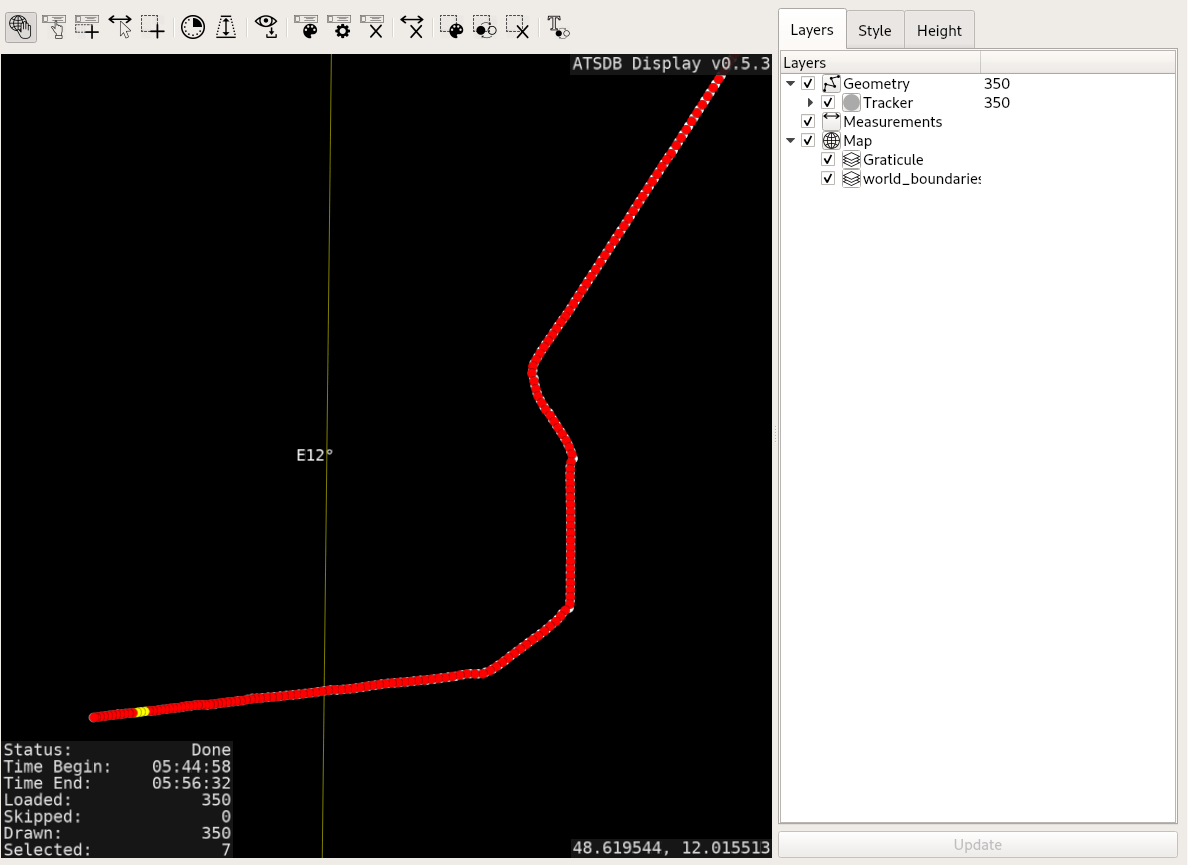
\includegraphics[width=18cm,frame]{../screenshots/view_points_osgview_selected.png}
  \caption{View Points OSGView: Selected View Point}
\end{figure}

Loaded data is presented as always and can be adapted to a users needs. After loading, the presented data is centered/zoomed according to the 'position\_latitude', 'position\_longitude', 'position\_window\_latitude', 'position\_window\_longitude' attributes. If these are not set, the center/zoom is adapted to encompass all of the loaded data.

\subsection{After Selection}

After data loading, the application can be used as in any other situation, therefore changing filters, adapting the OSGView style or re-loading the dataset is possible.

\subsection{Assessment}

In the 'View Points' tab, after assessing the view point, a user can add a comment and change the status to annotate the view point with additional information. \\

After this e.g. the next view point can be selected.
